% !TeX root = prob.tex

\section{Gambler's Ruin}\label{s.gamblers}

\textbf{Problem} Two players $A$ and $B$ compete in a contest. There is an initial finite capital of $n$ units: $A$ has $i$ and $B$ has $n-i$. They repeatedly play a game where the probability that $A$ wins is $p$ and the probability that $B$ wins is $q=1-p$. The loser gives one unit to the winner. When one player has all $n$ units the contest is terminated and that player is declared the winner.
\begin{enumerate}
\item Given initial parameters $(p, n, i)$, what is the probability that $A$ wins?
\item What is the expected duration of the game?
\end{enumerate}
\begin{center}
\begin{tikzpicture}[scale=1.2]
\draw (0,0) node[above left] {$A$} -- 
      (10,0) node[above right] {$B$};
\foreach \x in {0,1,2,3,4,5,6,7,8,9,10} {
  \draw (\x,0) -- +(0,4pt);
  \node at (\x,-10pt) { $\x$ };
}
\node at (4,-9mm) {$i$};
\node at (10,-9mm) {$n$};
\draw[fill] (4,7mm) circle[radius=1pt];
\draw[->] (4,7mm) -- node[above] {$q$} +(-1,0);
\draw[->] (4,7mm) -- node[above] {$p$} +(1,0);
\end{tikzpicture}
\end{center}
The most extensive presentation the gambler's ruin is in 
\cite[Chapter~2]{privault} which includes the solution to the expected duration of the contest. Note that Privault asks for the probability that $A$ is ruined, that is, that $B$ wins. I follow other references which ask for $A$'s probability of winning.

\subsection{Theoretical results}

Given $(p,n,i)$ the probability that $A$ wins the contest is:
\[
P_A(p, n, i) = \left(\frac{1-r^{i}}{1-r^n}\right)\,,
\]
where $r=q/p$. By symmetry, the probability that $B$ wins is:
\[
P_B(p, n, i) = \left(\frac{1-(1/r)^{n-i}}{1-(1/r)^{n}}\right)\,.
\]

There are separate solutions for $p\neq 1/2$ and $p=1/2$. For $p\neq 1/2$ the expected duration of the contest is:
\[
E_{\mathit{duration}}(p,n,i)=\frac{1}{q-p}\left(i-n
\frac{1-r^k}{1-r^n}\right)\,.
\]
For $p=1/2$ the expected duration of the contest is:
\[
E_{\mathit{duration}}(p,n,i)=i(n-1)\,.
\]
Of course the duration does not depend on which player wins. If $A$ wins, the contest terminates for $B$ also, and conversely.

\subsection{Program structure}

\verb+configuration.py+ contains declarations of variables which are intended to be constant.

\verb+gambler_plot.py+ contains the functions for plotting the histogram of the durations of all the runs of the simulation. If the simulations are run for multiple probabilities or initial values, a graph of the proportion of wins is also displayed.

\verb+gamblers_ruin.py+ is the main program which obtains the parameters, runs the simulations, prints the output and calls the plotting functions.

\subsection{Running the simulations}

The program asking the user how to run the simulations and then runs them in a loop. You can run the same simulation again with the saved parameters, enter new parameters, or run a sequence of simulations for a range of probabilities or initial values. Here is an output for $10000$ simulations:
\begin{verbatim}
Probability = 0.45, capital = 20, initial = 8
Wins = 789, losses = 9211, limits exceeded = 0
Proportion of wins     = 0.0789
Probability of winning = 0.0732
Average duration  = 65
Expected duration = 65
\end{verbatim}
A graph of the proportion of wins and the histogram of the durations are shown in Figures~\ref{f.gambler-hist1}, \ref{f.gambler-hist2}. The vertical lines are the average durations.

\begin{figure}
\begin{center}
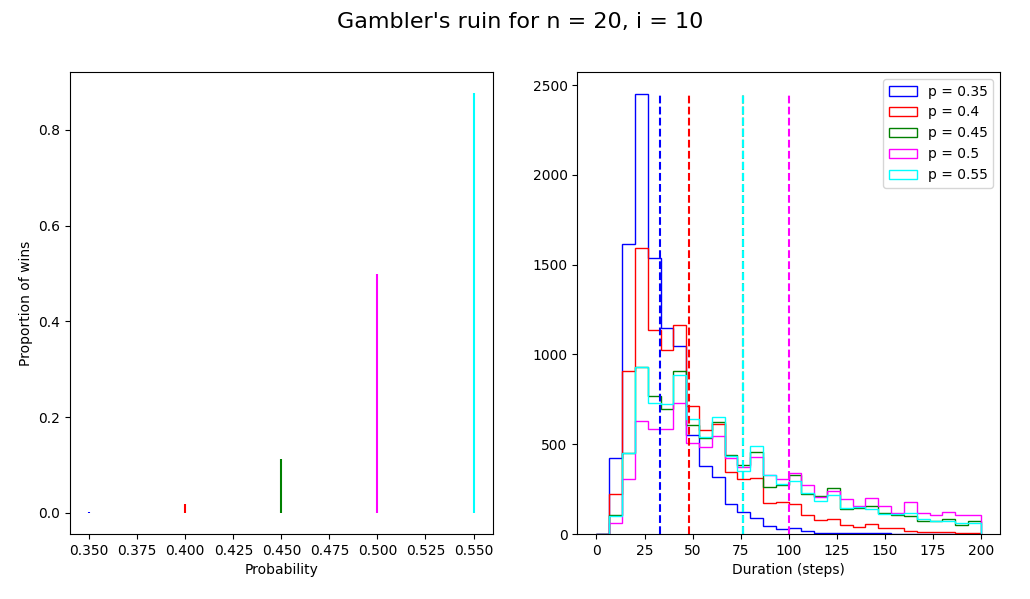
\includegraphics[width=\textwidth]{gamblers-ruin-01}
\caption{Proportion of wins and histogram for $n=20, i=10$ and multiple probabilities}\label{f.gambler-hist1}
\end{center}
\end{figure}

\begin{figure}
\begin{center}
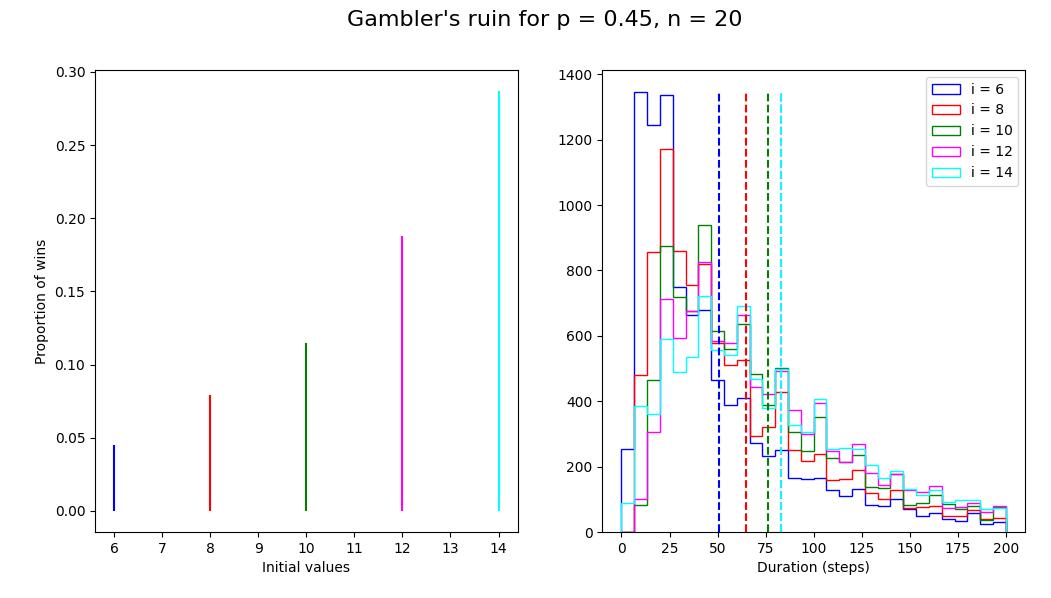
\includegraphics[width=\textwidth]{gamblers-ruin-02}
\caption{Proportion of wins and histogram for $p=0.45, n=20$ and multiple initial values}\label{f.gambler-hist2}
\end{center}
\end{figure}
